\documentclass[11pt]{article}
\usepackage{amsmath, amssymb, physics, geometry, graphicx, xcolor}
\usepackage{hyperref}
\usepackage{cite}
\usepackage{tikz}
\usetikzlibrary{arrows.meta, decorations.pathmorphing, positioning}
\geometry{a4paper, margin=1in}

\setlength{\parskip}{1em}

\title{A Holographic View of the QCD Axion}
\author{Tony Gherghetta \\ from KAIST Hep-Th seminar}
\date{August 4, 2026}

\begin{document}

\maketitle

\begin{abstract}
These notes meticulously transcribe a seminar on combining warped extra dimensions with the Peccei-Quinn mechanism to solve the strong CP problem. The framework maps the axion quality problem into a holographic AdS$_5$ setting via the AdS/CFT dictionary. It explicitly explores symmetry breaking mechanisms across the bulk and branes, the 4D/5D duality of gauge axions, and investigates whether 5D small instantons can dynamically enhance the QCD axion mass.
\end{abstract}

\section{The Strong CP Problem}
The strong CP problem originates from the CP-odd topological term in the QCD Lagrangian:
\begin{equation}
    \mathcal{L}_{\text{QCD}} \supset \theta_{\text{QCD}} \frac{\alpha_s}{8\pi} G_{\mu\nu}^a \tilde{G}^{a\mu\nu}.
\end{equation}
Because of the chiral anomaly, the physically observable parameter is basis independent and must include the phases of the quark mass matrix:
\begin{equation}
    \bar{\theta} = \theta_{\text{QCD}} + \arg(\det M_q)
\end{equation}
This effective term generates an observable effect on the neutron electric dipole moment, given by $d_n \simeq (5 \times 10^{-16} e\text{-cm}) \bar{\theta}$. Experimental bounds demand that $\bar{\theta} \le 10^{-10}$. 

Why is it so small? As Witten (1979) \cite{witten1979} noted, this extreme fine-tuning does not appear to be "anthropic"—our universe is perfectly possible for $\bar{\theta} \sim \mathcal{O}(1)$. 

\section{The Peccei-Quinn Mechanism and KSVZ Model}
To solve this dynamically, the Peccei-Quinn (PQ) mechanism introduces a spontaneously broken global $U(1)_{\text{PQ}}$ symmetry \cite{pecceiquinn1977, weinberg1978, wilczek1978}. 

The axion field is parameterized via a complex scalar:
\begin{equation}
    \Phi = \frac{1}{\sqrt{2}}(f_a + \rho) e^{i a / f_a}
\end{equation}
Below the symmetry breaking scale, the radial mode is integrated out, leaving the effective Lagrangian:
\begin{equation}
    \mathcal{L} = \frac{1}{2}(\partial_\mu a)^2 + \frac{\alpha_s}{8\pi} \left(\frac{a}{f_a} + \bar{\theta}\right) G\tilde{G} + \frac{1}{4} a g_{a\gamma\gamma} F\tilde{F} + \frac{1}{f_a} J^\mu \partial_\mu a
\end{equation}
In the KSVZ framework \cite{kim1979, shifman1980}, the scalar potential is $V(\Phi) = -m_{\text{PQ}}^2 |\Phi|^2 + \lambda_{\text{PQ}} |\Phi|^4$, yielding a VEV of $\langle \Phi \rangle = f_a / \sqrt{2}$, where $f_a = \sqrt{m_{\text{PQ}}^2 / \lambda_{\text{PQ}}}$. Heavy quarks acquire a mass via the Yukawa coupling:
\begin{equation}
    \Delta \mathcal{L} = y \bar{\psi} \Phi \psi + \text{h.c.} \implies m_\psi \sim y \frac{f_a}{\sqrt{2}}
\end{equation}
Integrating out these Dirac fermions naturally generates the dimension-5 axion-gluon coupling. 

\section{The Axion Quality Problem and Guiding Questions}
Gravitational violation of the global $U(1)_{\text{PQ}}$ symmetry induces higher-dimensional, Planck-suppressed operators of the form:
\begin{equation}
    \Delta \mathcal{L}_{\text{grav}} = \frac{|C_n| e^{i\delta_n}}{M_P^{n-4}} \Phi^n + \text{h.c.}
\end{equation}
This modifies the axion potential to:
\begin{equation}
    V(a) \simeq V_{\text{QCD}}(a) - \frac{|C_n| f_a^n}{M_P^{n-4}} \cos\left(\frac{n a}{f_a} + \delta_n\right)
\end{equation}
Because of the arbitrary phase $\delta_n$, the minimum of the potential shifts such that $\theta_{\text{eff}} \neq 0$. To solve the axion quality problem, these terms must be suppressed to a very high order ($n \ge 10$) \cite{randall1992, dobrescu1996, cheng2001}. 

This leads to three fundamental questions:
\begin{enumerate}
    \item What is the origin of the PQ breaking potential and the spontaneous breaking scale $f_a$?
    \item How to solve the axion quality problem? Is there a connection to GUT or SUSY?
    \item Can the QCD axion mass be different from $m_{a,\text{QCD}}$?
\end{enumerate}
To address these questions, we use a warped dimension.


\section{Warped Extra Dimensions (AdS$_5$)}
To generate a hierarchy of scales and small couplings, we introduce a warped 5D dimension \cite{cox2019}. The 5D metric is defined by:
\begin{equation}
    ds^2 = \frac{1}{(kz)^2} \left( \eta_{\mu\nu} dx^\mu dx^\nu + dz^2 \right) = g_{MN} dx^M dx^N
\end{equation}
where the IR and UV scales are related by $\Lambda_{\text{IR}} = \Lambda_{\text{UV}} e^{-\pi k R}$. 

\begin{figure}[h]
    \centering
    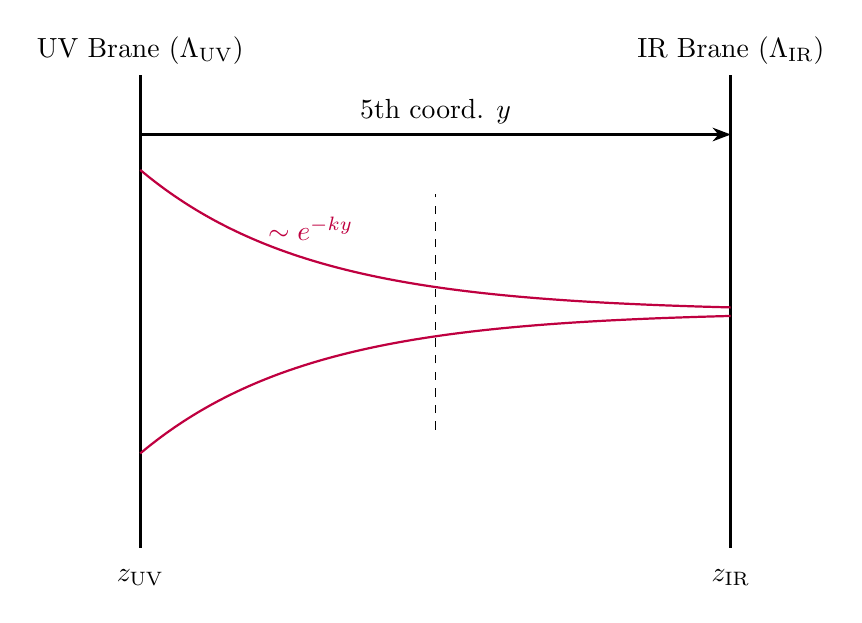
\begin{tikzpicture}[scale=1.5]
        % Branes
        \draw[very thick] (0, -2) -- (0, 2) node[above] {UV Brane ($\Lambda_{\text{UV}}$)};
        \draw[very thick] (5, -2) -- (5, 2) node[above] {IR Brane ($\Lambda_{\text{IR}}$)};
        
        % 5th dimension axis
        \draw[-{Stealth}, thick] (0, 1.5) -- (5, 1.5) node[midway, above] {5th coord. $y$};
        
        % Wavefunction exponential decay profile
        \draw[thick, purple, smooth, domain=0:5, samples=100] 
            plot (\x, {1.2*exp(-0.7*\x)});
        \draw[thick, purple, smooth, domain=0:5, samples=100] 
            plot (\x, {-1.2*exp(-0.7*\x)});
            
        % Labels and annotations
        \node[right, purple] at (1, 0.7) {$\sim e^{-ky}$};
        \node[below] at (0, -2.1) {$z_{\text{UV}}$};
        \node[below] at (5, -2.1) {$z_{\text{IR}}$};
        
        % Intermediate dashed marker
        \draw[dashed] (2.5, -1) -- (2.5, 1);
    \end{tikzpicture}
    \caption{Warped AdS$_5$ geometry showing the UV and IR branes with a localized bulk wavefunction.}
    \label{fig:warped_geometry}
\end{figure}

\subsection{Symmetry Breaking in the Bulk}
The bulk scalar field $\Phi = \frac{1}{\sqrt{2}} \eta(z) e^{i a(x,z) / f_a}$ has a bulk mass of $m_\Phi^2 = \Delta(\Delta-4)k^2$. Its background VEV profile is parameterized to capture two distinct symmetry-breaking mechanics:
\begin{equation}
    \eta(z) = k^{3/2} \left( v(kz)^{\Delta-4} + \sigma(kz)^\Delta \right)
\end{equation}
\begin{itemize}
    \item $v$: Governs the explicit breaking due to gravity, localized on the UV brane.
    \item $\sigma$: Governs the spontaneous breaking of the axion symmetry propagating through the bulk.
\end{itemize}

\subsection{No UV PQ-Breaking ($v = 0$)}
If there is no explicit UV breaking ($v = 0$), the global shift symmetry $a^{(0)}(x^\mu) \to a^{(0)}(x^\mu) + \text{const}$ is exact, resulting in a perfectly massless axion. The decay constant evaluates to:
\begin{equation}
    f_a^{(0)}(z) = f_a^{(0)}(z_{\text{UV}}) \simeq \frac{z_{\text{IR}}}{\sigma_0} \sqrt{\Delta-1} \quad (z_{\text{IR}} \gg z_{\text{UV}})
\end{equation}

\subsection{UV PQ-Breaking ($v \neq 0$)}
When gravity induces explicit breaking on the UV brane, the potential includes an interaction:
\begin{equation}
    U_{\text{UV}}(\Phi) \supset -2 l_{\text{UV}} k^{5/2} \eta \cos\left(\frac{a}{f_a}\right) = -2 l_{\text{UV}} k^{5/2} \eta \left(1 - \frac{a^2}{2f_a^2} + \dots \right)
\end{equation}
This explicitly breaks the symmetry, suppressing the axion decay constant such that:
\begin{equation}
    f_a^{(0)}(z_{\text{UV}}) \simeq \frac{4 z_{\text{IR}} \sqrt{\Delta-1}}{l_{\text{UV}}} (\Delta-2) \left(\frac{z_{\text{UV}}}{z_{\text{IR}}}\right)^\Delta \quad (z_{\text{UV}} \ll z_{\text{IR}}, \Delta > 4)
\end{equation}
The resulting UV axion mass is heavily suppressed for large scaling dimension $\Delta$:
\begin{equation}
    (m_a^{(UV)})^2 = \frac{6 l_{\text{UV}} v (\Delta-2)}{k(\Delta-4+l_{\text{UV}})} \left( \frac{k\sqrt{\Delta-1}}{v} \right)^\Delta \left(\frac{f_a}{\Lambda_{\text{UV}}}\right)^{\Delta-4} f_a^2
\end{equation}
Requiring $(m_a^{(UV)})^2 \le 10^{-10} (m_a^{(QCD)})^2$ guarantees protection for $\Delta \ge 10$.

\section{AdS/CFT Dictionary: 4D and 5D Duality}
The holographic interpretation provides a powerful duality mapping between 5D AdS space and strongly coupled 4D gauge theories. The explicit AdS/CFT dictionary is:
\begin{itemize}
    \item \textbf{5D local gauge symmetry} $\leftrightarrow$ \textbf{4D global symmetry}
    \item \textbf{5D field $\Phi$} with $m_\Phi^2 = \Delta(\Delta-4)k^2$ $\leftrightarrow$ \textbf{4D operator $\mathcal{O}$} with $\dim \mathcal{O} = \Delta$
    \item \textbf{5D scale} $\Lambda_{\text{UV}} e^{-\pi k R} = \Lambda_{\text{IR}}$ $\leftrightarrow$ \textbf{4D scale} $\Lambda_{\text{IR}} = \Lambda_{\text{UV}} e^{-\frac{8\pi^2}{b_{\text{CFT}} g^2}}$
\end{itemize}

Under this holographic interpretation, the 5D Axion corresponds exactly to a 4D composite axion featuring an accidental global PQ symmetry \cite{kim1985, choikim1985}. The elementary PQ scalar becomes a dynamical fermion condensate $\langle \bar{\psi}\psi\dots\psi \rangle$. Consequently, the axion quality problem maps directly between dimensions:
\begin{equation}
    \frac{c_n}{M_P^{n-4}} \Phi^n \leftrightarrow \frac{c_\Delta}{M_P^{\Delta-4}} \mathcal{O} \sim \frac{c_\Delta}{M_P^{\Delta-4}} (\psi_i \psi_j \dots \psi_k) \quad (\Delta \ge 10)
\end{equation}
These models better incorporate SM features by introducing naturally massless exotic quarks, making the SM part of the strong dynamics, and providing a connection to GUT/supersymmetry breaking \cite{gherghetta2025_08888, sato2025, gherghetta2025_21813}.

\section{5D Gauge Axion in Warped GUT}
In a warped Grand Unified Theory (GUT) \cite{choi2025_15666}, the SM fermions $\{10_i, \bar{5}_i\}$ and Higgs $\{24_\Phi, 5_H, \bar{5}_H\}$ are embedded in $SU(5)_{\text{GUT}} \times U(1)_{\text{PQ}}$. The fields are represented by $A_M^{(\text{GUT})}$ and $A_M^{(\text{PQ})}$.

The QCD axion resides in the 5th component, defined by $\theta(x) = \frac{a(x)}{f_a} = \oint dy A_5(x,y)$. This guarantees an exact shift symmetry under $U(1)_c^{(1)}$:
\begin{equation}
    A^{(\text{PQ})} \to A^{(\text{PQ})} + \Lambda_c^{(1)}, \quad d\Lambda_c^{(1)} = 0 \implies A_5^{(\text{PQ})} \to A_5^{(\text{PQ})} + \lambda
\end{equation}
The axion quality violation due to brane-localized charged matter takes the suppressed form:
\begin{equation}
    \Delta V(\theta) \sim M_5^4 e^{-2\pi k R_1} e^{-\pi R \sqrt{M_5^2 + 4k^2}} \cos\left(\frac{q\theta}{2} + \delta\right)
\end{equation}

\subsection{Gauge Coupling Unification}
In warped AdS$_5$, the gauge coupling unification is preserved with a logarithmic scaling:
\begin{equation}
    \frac{2\pi}{\alpha_i(\mu)} = \frac{2\pi}{\alpha_i(m_{\text{KK}})} - (b_i^{(\text{SM})} - b_i^{(\text{CFT})}) \log\left(\frac{m_{\text{KK}}}{\mu}\right)
\end{equation}
Using MSSM beta functions $(3, -1, -33/5)$, the warped 5D gauge axion is highly compatible with grand unification scales $f_a \ge 10^9$ GeV \cite{benabou2025}.

\subsection{Possible Dual 4D Description}
This setup boasts a precise 4D dual mapping:
\begin{itemize}
    \item 5D bulk $U(1)$ $\leftrightarrow$ 4D global $U(1)_B$
    \item IR breaking of $U(1)$ ($\int_{\text{UV}}^{\text{IR}} dy A_5$) $\leftrightarrow$ Spontaneously broken $U(1)_B$ ($\langle B \rangle \neq 0, \arg(\mathcal{B})$)
    \item 5D locality (no charged matter) $\leftrightarrow$ $\dim B \sim N \to \infty$
\end{itemize}
The PQ symmetry is spontaneously broken by an infinite dimension operator. A wrapped D3 particle is charged under $U(1) = \text{baryon}$. For 4D SQCD where $N_f = N_c = N$, we have $\det M - B\bar{B} = \Lambda^{2N}$, with $U(1)_{\text{PQ}} = U(1)_B$ and $B \sim Q^N$.

\section{Enhancing the Axion Mass and Small Instantons}
The QCD axion mass is derived from the topological susceptibility $\mathcal{T}$:
\begin{equation}
    m_a^2 f_a^2 = \mathcal{T} \equiv -i \int d^4x \langle 0 | T\left[ \frac{\alpha_s}{8\pi} G\tilde{G}(x), \frac{\alpha_s}{8\pi} G\tilde{G}(0) \right] | 0 \rangle
\end{equation}
In the dilute instanton gas approximation:
\begin{equation}
    \mathcal{T} \propto \int \frac{d\rho}{\rho^5} C[3] \left(\frac{2\pi}{\alpha_s(1/\rho)}\right)^6 e^{-\frac{2\pi}{\alpha_s(1/\rho)}}
\end{equation}
Because QCD is asymptotically free, this is suppressed by fermion zero modes $(\rho m_f)^{N_f}$, yielding the standard mass
\begin{equation}
    m_{a,\text{QCD}}^2 = \frac{m_u m_d}{(m_u + m_d)^2} \frac{m_\pi^2 f_\pi^2}{f_a^2}.
\end{equation}
To enhance this mass, we can change the QCD coupling in the UV (via small instantons) or close fermion loops with Higgs configurations ($\kappa_f$).

\subsection{5D Small Instantons in Flat Space}
For flat 5D space $ds^2 = \eta_{\mu\nu} dx^\mu dx^\nu + dy^2$, the localized instanton profile is
\begin{equation}
    A_\mu^{(I)a}(x) = \frac{2 \eta_{a\mu\nu} (x-x_0)_\nu}{(x-x_0)^2 + \rho^2}
\end{equation}
$A_5^a = 0$ \cite{poppitz2002}. This gives a finite action $S_5^{(I)} = \frac{8\pi^2 R}{g_5^2} = \frac{2\pi}{\alpha_s}$. Including Kaluza-Klein fluctuations \cite{dienes1998}:
\begin{equation}
    S_{\text{eff}} = \frac{2\pi}{\alpha_s(1/R)} - 3\xi(R/\rho) \frac{R}{\rho} + b_0 \ln \frac{R}{\rho}
\end{equation}
The power-law term $(- \frac{R}{\rho})$ overcomes the suppression, allowing small 5D instantons to dominate for $1/R \gtrsim 100$ TeV \cite{gherghetta2020}. This holds up to $\Lambda_5 R \le \frac{6\pi}{\alpha_s}$.

\subsection{Holographic Obstruction in AdS$_5$}
When embedded in warped AdS$_5$ \cite{gherghetta2021}, the coupling behaves as:
\begin{equation}
    \frac{2\pi}{\alpha_s(1/\rho)} = \frac{2\pi}{\alpha_s(M_{\text{IR}})} - \left(b_0 + \frac{8\pi^2}{g_5^2 k}\right) \log\left(\frac{\rho^{-1}}{M_{\text{IR}}}\right)
\end{equation}
Applying the classical bulk profile
\begin{equation}
    A_\mu^{(cl)}(x,z) = -i (\partial_\mu \Omega) \Omega^{-1} \frac{x^2}{x^2 + \rho^2},
\end{equation}
the action resolves to
\begin{equation}
    S_5^{(I)} = \frac{8\pi^2}{g_5 k} \log \frac{M_{\text{UV}}}{M_{\text{IR}}}.
\end{equation}

Holographically, the CFT constituents must be bifundamental colored matter. Two possibilities exist:
\begin{enumerate}
    \item \textbf{Colored fermion constituents:} This results directly in chiral suppression from CFT fermions $(\rho M_{\text{IR}})^{b_{\text{CFT}}}$, meaning no axion mass enhancement.
    \item \textbf{Colored scalar constituents:} This bypasses chiral suppression and enhances the mass. However, topological charge conservation dictates that no localized instanton exists for this boundary condition.
\end{enumerate}

\subsection{Holographic Obstruction in AdS$_5$}
When embedded in warped AdS$_5$, we must evaluate the QCD instantons in the 5D bulk \cite{gherghetta2021}. The coupling behaves as:
\begin{equation}
    \frac{2\pi}{\alpha_s(1/\rho)} = \frac{2\pi}{\alpha_s(M_{\text{IR}})} - \left(b_0 + \frac{8\pi^2}{g_5^2 k}\right) \log\left(\frac{\rho^{-1}}{M_{\text{IR}}}\right)
\end{equation}
Applying the classical 5D test profile $A_\mu^{(cl)}(x,z) = -i (\partial_\mu \Omega) \Omega^{-1} \frac{x^2}{x^2 + \rho^2}$ (where $\Omega \in SU(2)$) and $A_5(x,z) = 0$, we integrate the classical field strength over the warped bulk to find the finite action:
\begin{align}
    S_5^{(I)}[A_\mu^{(cl)}(x,z)] &= -\frac{1}{2g_5^2} \int d^4x \int_{1/M_{\text{UV}}}^{1/M_{\text{IR}}} dz \sqrt{g} \text{Tr} \left[ G_{MN}^{(cl)} G^{MN(cl)} \right] \nonumber \\
    &= \frac{8\pi^2}{g_5^2 k} \log \frac{M_{\text{UV}}}{M_{\text{IR}}} = \frac{2\pi}{\alpha_s(M_{\text{IR}})} \neq \frac{2\pi}{\alpha_s(1/\rho)}
\end{align}
Because the result is fixed at $\frac{2\pi}{\alpha_s(M_{\text{IR}})}$ and does not equal $\frac{2\pi}{\alpha_s(1/\rho)}$, the instanton action fails to scale with the instanton size $\rho$. 

Holographically, this indicates a fundamental obstruction. The CFT constituents must be bifundamental colored matter. There are two possibilities:
\begin{enumerate}
    \item \textbf{Colored fermion constituents:} This results directly in chiral suppression from CFT fermions $(\rho M_{\text{IR}})^{b_{\text{CFT}}}$, meaning no axion mass enhancement.
    \item \textbf{Colored scalar constituents:} This bypasses chiral suppression and enhances the mass. However, strict topological charge conservation dictates that no localized instanton exists for this boundary condition.
\end{enumerate}

\section{Summary}
\begin{itemize}
    \item The axion quality problem can be fully solved in a 5D warped dimension, perfectly dual to a 4D composite axion with an accidental PQ symmetry.
    \item This warped framework elegantly explains fermion mass hierarchies and naturally incorporates GUT and axion isocurvature scales.
    \item Flat 5D small instantons can enhance the axion mass while protecting the strong CP solution. However, a warped AdS$_5$ instantiation faces an inescapable obstruction dictated by the nature of colored constituents in the dual CFT.
\end{itemize}

\clearpage
\addcontentsline{toc}{section}{References}
%\bibliographystyle{alpha}
\bibliographystyle{amsalpha}
\bibliography{references}

\end{document}